\documentclass[11pt]{scrreprt}
%%fakesection Load packages
% These are evan.sty
\usepackage{amsmath,amssymb,amsthm}
\usepackage{mathrsfs}
\usepackage[usenames,svgnames,dvipsnames]{xcolor}
\usepackage{hyperref}
\usepackage[nameinlink]{cleveref}
\usepackage{textcomp}
\usepackage{enumerate}
\usepackage[obeyFinal,textsize=scriptsize,shadow]{todonotes}
\usepackage{mathtools}
\usepackage{microtype}

\usepackage[normalem]{ulem}
\usepackage{stmaryrd}
\usepackage{wasysym}
\usepackage{multirow}
\usepackage{prerex}

%%fakesection evan.sty macros
%Small commands
\newcommand{\cbrt}[1]{\sqrt[3]{#1}}
\newcommand{\floor}[1]{\left\lfloor #1 \right\rfloor}
\newcommand{\ceiling}[1]{\left\lceil #1 \right\rceil}
\newcommand{\mailto}[1]{\href{mailto:#1}{\texttt{#1}}}
\newcommand{\ol}{\overline}
\newcommand{\ul}{\underline}
\newcommand{\wt}{\widetilde}
\newcommand{\wh}{\widehat}
\newcommand{\eps}{\varepsilon}
%\renewcommand{\iff}{\Leftrightarrow}
%\renewcommand{\implies}{\Rightarrow}
\newcommand{\vocab}[1]{\textbf{\color{blue} #1}}
\newcommand{\catname}{\mathsf}
\newcommand{\hrulebar}{
  \par\hspace{\fill}\rule{0.95\linewidth}{.7pt}\hspace{\fill}
  \par\nointerlineskip \vspace{\baselineskip}
}
\newcommand{\half}{\frac{1}{2}}

%For use in author command
\newcommand{\plusemail}[1]{\\ \normalfont \texttt{\mailto{#1}}}

%More commands and math operators
\DeclareMathOperator{\cis}{cis}
\DeclareMathOperator*{\lcm}{lcm}
\DeclareMathOperator*{\argmin}{arg min}
\DeclareMathOperator*{\argmax}{arg max}

%Convenient Environments
\newenvironment{soln}{\begin{proof}[Solution]}{\end{proof}}
\newenvironment{parlist}{\begin{inparaenum}[(i)]}{\end{inparaenum}}
\newenvironment{gobble}{\setbox\z@\vbox\bgroup}{\egroup}

%Inequalities
\newcommand{\cycsum}{\sum_{\mathrm{cyc}}}
\newcommand{\symsum}{\sum_{\mathrm{sym}}}
\newcommand{\cycprod}{\prod_{\mathrm{cyc}}}
\newcommand{\symprod}{\prod_{\mathrm{sym}}}

%From H113 "Introduction to Abstract Algebra" at UC Berkeley
\newcommand{\CC}{\mathbb C}
\newcommand{\FF}{\mathbb F}
\newcommand{\NN}{\mathbb N}
\newcommand{\QQ}{\mathbb Q}
\newcommand{\RR}{\mathbb R}
\newcommand{\ZZ}{\mathbb Z}
\newcommand{\charin}{\text{ char }}
\DeclareMathOperator{\sign}{sign}
\DeclareMathOperator{\Aut}{Aut}
\DeclareMathOperator{\Inn}{Inn}
\DeclareMathOperator{\Syl}{Syl}
\DeclareMathOperator{\Gal}{Gal}
\DeclareMathOperator{\GL}{GL} % General linear group
\DeclareMathOperator{\SL}{SL} % Special linear group

%From Kiran Kedlaya's "Geometry Unbound"
\newcommand{\abs}[1]{\left\lvert #1 \right\rvert}
\newcommand{\norm}[1]{\left\lVert #1 \right\rVert}
\newcommand{\dang}{\measuredangle} %% Directed angle
\newcommand{\ray}[1]{\overrightarrow{#1}} 
\newcommand{\seg}[1]{\overline{#1}}
\newcommand{\arc}[1]{\wideparen{#1}}

%From M275 "Topology" at SJSU
\newcommand{\id}{\mathrm{id}}
\newcommand{\taking}[1]{\xrightarrow{#1}}
\newcommand{\inv}{^{-1}}

%From M170 "Introduction to Graph Theory" at SJSU
\DeclareMathOperator{\diam}{diam}
\DeclareMathOperator{\ord}{ord}
\newcommand{\defeq}{\overset{\mathrm{def}}{=}}

%From the USAMO .tex filse
\newcommand{\st}{^{\text{st}}}
\newcommand{\nd}{^{\text{nd}}}
\renewcommand{\th}{^{\text{th}}}
\newcommand{\dg}{^\circ}
\newcommand{\ii}{\item}

% From Math 55 and Math 145 at Harvard
\newenvironment{subproof}[1][Proof]{%
\begin{proof}[#1] \renewcommand{\qedsymbol}{$\blacksquare$}}%
{\end{proof}}

\newcommand{\liff}{\leftrightarrow}
\newcommand{\lthen}{\rightarrow}
\newcommand{\opname}{\operatorname}
\newcommand{\surjto}{\twoheadrightarrow}
\newcommand{\injto}{\hookrightarrow}
\newcommand{\On}{\mathrm{On}} % ordinals
\DeclareMathOperator{\img}{im} % Image
\DeclareMathOperator{\Img}{Im} % Image
\DeclareMathOperator{\coker}{coker} % Cokernel
\DeclareMathOperator{\Coker}{Coker} % Cokernel
\DeclareMathOperator{\Ker}{Ker} % Kernel
\DeclareMathOperator{\rank}{rank}
\DeclareMathOperator{\Spec}{Spec} % spectrum
\DeclareMathOperator{\Tr}{Tr} % trace
\DeclareMathOperator{\pr}{pr} % projection
\DeclareMathOperator{\ext}{ext} % extension
\DeclareMathOperator{\pred}{pred} % predecessor
\DeclareMathOperator{\dom}{dom} % domain
\DeclareMathOperator{\ran}{ran} % range
\DeclareMathOperator{\Hom}{Hom} % homomorphism
\DeclareMathOperator{\End}{End} % endomorphism

% Things Lie
\newcommand{\kb}{\mathfrak b}
\newcommand{\kg}{\mathfrak g}
\newcommand{\kh}{\mathfrak h}
\newcommand{\kn}{\mathfrak n}
\newcommand{\ku}{\mathfrak u}
\newcommand{\kz}{\mathfrak z}
\DeclareMathOperator{\Ext}{Ext} % Ext functor
\DeclareMathOperator{\Tor}{Tor} % Tor functor
\newcommand{\gl}{\opname{\mathfrak{gl}}} % frak gl group
\renewcommand{\sl}{\opname{\mathfrak{sl}}} % frak gl group

% More script letters etc.
\newcommand{\SA}{\mathscr A}
\newcommand{\SB}{\mathscr B}
\newcommand{\SC}{\mathscr C}
\newcommand{\SD}{\mathscr D}
\newcommand{\SF}{\mathscr F}
\newcommand{\SG}{\mathscr G}
\newcommand{\SH}{\mathscr H}
\newcommand{\OO}{\mathcal O}

%% Napkin commands
\newcommand{\prototype}[1]{
	\emph{{\color{red} Prototypical example for this section:} #1} \par\medskip
}
\newenvironment{moral}{%
	\begin{mdframed}[linecolor=green!70!black]%
	\bfseries\color{green!70!black}}%
	{\end{mdframed}}

%%% END EXCERPT OF EVAN.STY
%%fakesection Commutative diagrams
\usepackage{diagrams}
\newarrow{Inj}C--->
\newarrow{Surj}----{>>}
\newarrow{Proj}----{>>}
\newarrow{Embed}>--->
\newarrow{Incl}C--->
\newarrow{Mapsto}|--->
\newarrow{Isom}<--->
\newarrow{Dotted}....>
\newarrow{Dashed}{}{dash}{}{dash}>
\newarrow{Line}-----
\usepackage{tikz-cd}
\usetikzlibrary{decorations.pathmorphing}
\tikzcdset{row sep/normal=3.14em,column sep/normal=3.14em}

%%fakesection Page layout
\usepackage[headsepline]{scrlayer-scrpage}
\renewcommand{\headfont}{}
\addtolength{\textheight}{3.14cm}
\setlength{\footskip}{0.5in}
\setlength{\headsep}{10pt}
\ihead{Evan Chen}
\automark{section}
\chead{}
\ohead{\headmark}
\cfoot{\pagemark}

%%fakesection Fancy section and chapter heads
\addtokomafont{chapterprefix}{\raggedleft}
\renewcommand*{\sectionformat}{\color{purple}\S\thesection\autodot\enskip}

\RedeclareSectionCommand[beforeskip=0.5em]{chapter}
\renewcommand*{\chapterformat}{%
\mbox{\scalebox{1.5}{\chapappifchapterprefix{\nobreakspace}}%
\scalebox{2.718}{\color{purple}\thechapter\autodot}\enskip}}

\addtokomafont{partprefix}{\rmfamily}
\renewcommand*{\partformat}{\color{purple}\scalebox{2.5}{\thepart}%
	\enlargethispage{2em}}
\newcommand{\problemhead}{Problems to think about}

%%fakesection Mini ToC
\usepackage[tight]{minitoc}
\noptcrule
\mtcsetfont{parttoc}{section}{\small\rmfamily\upshape\mdseries}
\renewcommand*{\partheadstartvskip}{}
\renewcommand*{\partheadendvskip}{}
\renewcommand\beforeparttoc{\hspace{\fill}\rule{0.95\linewidth}{2pt}\hspace{\fill}}
\let\oldpart\part
\renewcommand{\part}[1]{\oldpart{#1}\parttoc\cleardoublepage}

%%fakesection SNSD
\newcommand{\snsd}[2][]%
{\includegraphics[#1]{/home/evan/Pictures/TopologicalGG/#2}}

%%fakesection Theorems
\usepackage{thmtools}
\usepackage[framemethod=TikZ]{mdframed}

\theoremstyle{definition}
\mdfdefinestyle{mdbluebox}{%
	roundcorner = 10pt,
	linewidth=1pt,
	skipabove=12pt,
	innerbottommargin=9pt,
	skipbelow=2pt,
	nobreak=true,
	linecolor=blue,
	backgroundcolor=TealBlue!5,
}
\declaretheoremstyle[
	headfont=\sffamily\bfseries\color{MidnightBlue},
	mdframed={style=mdbluebox},
	headpunct={\\[3pt]},
	postheadspace={0pt}
]{thmbluebox}

\mdfdefinestyle{mdrecbox}{%
	linewidth=0.5pt,
	skipabove=12pt,
	frametitleaboveskip=5pt,
	frametitlebelowskip=0pt,
	skipbelow=2pt,
	frametitlefont=\bfseries,
	innertopmargin=4pt,
	innerbottommargin=8pt,
	nobreak=true,
	linecolor=RawSienna,
	backgroundcolor=Salmon!5,
}
\declaretheoremstyle[
	headfont=\bfseries\color{RawSienna},
	mdframed={style=mdrecbox},
	headpunct={\\[3pt]},
	postheadspace={0pt},
]{thmrecbox}

\declaretheorem[%
style=thmbluebox,name=Theorem,numberwithin=section]{theorem}
\declaretheorem[style=thmbluebox,name=Lemma,sibling=theorem]{lemma}
\declaretheorem[style=thmbluebox,name=Proposition,sibling=theorem]{proposition}
\declaretheorem[style=thmbluebox,name=Corollary,sibling=theorem]{corollary}
\declaretheorem[style=thmrecbox,name=Example,sibling=theorem]{example}

\mdfdefinestyle{mdinlinebox}{%
	skipabove=8pt,
	linewidth=3pt,
	rightline=false,
	leftline=true,
	topline=false,
	bottomline=false,
	linecolor=gray,
	backgroundcolor=black!2
}
\declaretheoremstyle[
	headfont=\bfseries,
	bodyfont=\normalfont\small,
	spaceabove=0pt,
	spacebelow=0pt,
	mdframed={style=mdinlinebox}
]{thminlinebox}
\theoremstyle{theorem}
\declaretheorem[name=Question,sibling=theorem,style=thminlinebox]{ques}
\declaretheorem[name=Exercise,sibling=theorem,style=thminlinebox]{exercise}

\theoremstyle{definition}
\newtheorem{claim}[theorem]{Claim}
\newtheorem{definition}[theorem]{Definition}
\newtheorem{fact}[theorem]{Fact}
\newtheorem{remark}[theorem]{Remark}
\newtheorem{abuse}[theorem]{Abuse of Notation}

\newtheorem{problem}{Problem}[chapter]
\renewcommand{\theproblem}{\thechapter\Alph{problem}}
\newtheorem{sproblem}[problem]{Problem}
\newtheorem{dproblem}[problem]{Problem}
\renewcommand{\thesproblem}{\theproblem$^{\star}$}
\renewcommand{\thedproblem}{\theproblem$^{\dagger}$}
\newcommand{\listhack}{$\empty$\vspace{-2em}}

%%fakesection Answers
\usepackage{answers}
\Newassociation{hint}{answeritem}{tex/backmatter/all-hints}
\Newassociation{sol}{answeritem}{tex/backmatter/all-solns}
\renewcommand{\solutionextension}{out}
\renewenvironment{answeritem}[1]{\item[\bf #1.]}{}

%%fakesection Hot chili peppers
\reversemarginpar
\newcommand{\prechili}{\vspace*{0.3em}\hspace*{1.5em}}
\newcommand{\nochili}{\hspace*{1.5em}}
\newcommand{\chili}{
\includegraphics[width=1.5em]{media/chili.png}}
\newcommand{\gim}{\marginpar{\prechili\nochili\nochili\chili}}
\newcommand{\yod}{\marginpar{\prechili\nochili\chili\chili}}
\newcommand{\kurumi}{\marginpar{\prechili\chili\chili\chili}}

%%fakesection Table of contents
% First add ToC to ToC
\makeatletter
\usepackage{etoolbox}
\pretocmd{\tableofcontents}{%
  \if@openright\cleardoublepage\else\clearpage\fi
  \pdfbookmark[0]{\contentsname}{toc}%
}{}{}%
\makeatother
\setcounter{tocdepth}{1}
% Fix spacing issues in To
\usepackage[tocindentauto]{tocstyle}
\usetocstyle{KOMAlike}

%%fakesection Asymptote definitions
\usepackage{patch-asy}
\numberwithin{asy}{chapter}
\renewcommand{\theasy}{\thechapter\Alph{asy}}
\begin{asydef}
	import olympiad;
	import cse5;
	size(6cm);
	usepackage("amsmath");
	usepackage("amssymb");
	defaultpen(fontsize(11pt));
	pointfontsize=11;
	void bigbox(string L) {
		filldraw((-4,3)--(4,3)--(4,-3)--(-4,-3)--cycle,
			lightblue+opacity(0.2), black);
		label(L, (4,3), dir(-45));
	}
	void bigblob(string L) {
		filldraw((-4,3)..(-5,1)..(-4.7,0)..(-4.1,-2)..(-4,-3)
			..(-1,-3.3)..(1,-3.2)..(4,-3)
			..(4.3,-1)..(4.1,0.5)..(4,3)
			..(2,3.3)..(0,3.1)..(-3,2.9)..cycle,
			lightblue+opacity(0.2), black);
		label(L, (4,3), dir(5));
	}

	real[] default_ticks = {-4,-3,-2,-1,0,1,2.3,4};
	void cplane(real theta=-45, real[] T = default_ticks, real xmin = -4.5, real xmax = 4.5, real S = 3) {
		graph.xaxis("Re", xmin, xmax, graph.Ticks(format="%", Ticks=T, Size=S), Arrows);
		graph.yaxis("Im", xmin, xmax, graph.Ticks(format="%", Ticks=T, Size=S), Arrows);
		Drawing("0", origin, dir(theta));
		markscalefactor *= xmax;
	}

	pair opendot(pair P, pen p = defaultpen) {
		dot(P, p, UnFill);
		dot(P, p, Draw);
		return P;
	}
\end{asydef}
\def\asydir{asy}

%%fakesection Bibliography
\usepackage[backend=biber,style=alphabetic]{biblatex}
\DeclareLabelalphaTemplate{
	\labelelement{
		\field[final]{shorthand}
		\field{label}
		\field[strwidth=2,strside=left]{labelname}
	}
	\labelelement{
		\field[strwidth=2,strside=right]{year}    
	}
}
\DeclareFieldFormat{labelalpha}{\textbf{\scriptsize #1}}
\addbibresource{references.bib}
\addbibresource{images.bib}

%%fakesection Napkin Macros
\newcommand{\Zc}[1]{\ZZ_{#1}}
\newcommand{\Zm}[1]{\ZZ_{#1}^\times}
\newcommand{\pre}{^{\text{pre}}}
\newcommand{\normalin}{\trianglelefteq}
\newcommand{\triv}{\mathrm{triv}}
\newcommand{\largeotimes}[1]{\mathop{\otimes}\limits_{#1}}
\newcommand{\Mat}{\mathrm{Mat}}
\newcommand{\PGL}[1]{\mathbf{PGL}_{#1}(\CC)}

\DeclareMathOperator{\Stab}{Stab}
\DeclareMathOperator{\FixPt}{FixPt}
\DeclareMathOperator{\refl}{refl}
\DeclareMathOperator{\Fun}{Fun}
\DeclareMathOperator{\Irrep}{Irrep}
\DeclareMathOperator{\Res}{Res}
\DeclareMathOperator{\Reg}{Reg}
\DeclareMathOperator{\Classes}{Classes}
\newcommand{\FunCl}{\Fun_{\mathrm{class}}}
\newcommand{\Homrep}{\Hom_{\mathrm{rep}}}
\newcommand{\ab}{^\text{ab}} % abelianization
\DeclareMathOperator{\ev}{ev}
\DeclareMathOperator{\Wind}{\mathbf I}
\newcommand{\Ctriv}{\CC_{\mathrm{triv}}}
\newcommand{\Csign}{\CC_{\mathrm{sign}}}

% Alg geom macros
\newcommand{\VV}{\mathcal V}
\newcommand{\Vp}{\mathcal V_{\text{pr}}}
\newcommand{\Aff}{\mathbb A}
\newcommand{\II}{\mathcal I_{\text{rad}}}
\newcommand{\RP}{\mathbb{RP}}
\newcommand{\CP}{\mathbb{CP}}
\newcommand{\Cl}{\mathrm{Cl}}
\newcommand{\restrict}[1]{\bgroup\restriction_{#1}\egroup}
\DeclareMathOperator{\Opens}{OpenSets}
\DeclareMathOperator{\Proj}{Proj}
\DeclareMathOperator{\res}{res}
\newcommand{\mm}{\mathfrak m}
\newcommand{\sh}{^\mathrm{sh}}

\renewcommand{\Re}{\opname{Re}}
\renewcommand{\Im}{\opname{Im}}

%% Category Theory macros
\renewcommand{\AA}{\mathcal A}
\newcommand{\BB}{\mathcal B}
\newcommand{\obj}{\operatorname{obj}}
\newcommand{\op}{^{\mathrm{op}}}


\usepackage{tkz-graph}
\pgfarrowsdeclare{biggertip}{biggertip}{%
  \setlength{\arrowsize}{1pt}  
  \addtolength{\arrowsize}{.1\pgflinewidth}  
  \pgfarrowsrightextend{0}  
  \pgfarrowsleftextend{-5\arrowsize}  
}{%
  \setlength{\arrowsize}{1pt}  
  \addtolength{\arrowsize}{.1\pgflinewidth}  
  \pgfpathmoveto{\pgfpoint{-5\arrowsize}{4\arrowsize}}  
  \pgfpathlineto{\pgfpointorigin}  
  \pgfpathlineto{\pgfpoint{-5\arrowsize}{-4\arrowsize}}  
  \pgfusepathqstroke  
}  
\tikzset{
	EdgeStyle/.style = {>=biggertip}
}

\usepackage[all,cmtip,2cell]{xy}
\UseTwocells
\newcommand\nattfm[5]{\xymatrix@C+2pc{#1 \rtwocell<4>^{#2}_{#4}{\; #3} & #5}}

%% Alg Top macros
\DeclareMathOperator{\Cells}{Cells}
\newcommand{\HdR}{H_{\mathrm{dR}}}

%% Alg NT macros
\renewcommand{\aa}{\mathfrak a}
\newcommand{\bb}{\mathfrak b}
\newcommand{\pp}{\mathfrak p}
\newcommand{\qq}{\mathfrak q}

\newcommand{\Frob}{\mathrm{Frob}}
\DeclareMathOperator{\Norm}{N}
\DeclareMathOperator{\Ram}{Ram}
\newcommand{\TrK}{\Tr_{K/\QQ}}
\newcommand{\NK}{\Norm_{K/\QQ}}
\newcommand{\kf}{\mathfrak f}
\newcommand{\kP}{\mathfrak P}
\newcommand{\kQ}{\mathfrak Q}

%% Diff geo macros
\newcommand{\ee}{\mathbf e}
\newcommand{\fpartial}[2]{\frac{\partial #1}{\partial #2}}

%% ST macros
\newcommand{\CH}{\mathsf{CH}}
\newcommand{\ZFC}{\mathsf{ZFC}}

\newcommand{\Name}{\text{Name}}
\newcommand{\Po}{\mathbb P}
\newcommand{\nrank}{\opname{n-rank}} % ranks
\newcommand{\PP}{\mathcal P}

\newcommand{\EmptySet}{\mathrm{EmptySet}}
\newcommand{\PowerSet}{\mathrm{PowerSet}}
\newcommand{\Pairing}{\mathrm{Pairing}}
\newcommand{\Infinity}{\mathrm{Infinity}}
\newcommand{\Extensionality}{\mathrm{Extensionality}}
\newcommand{\Foundation}{\mathrm{Foundation}}
\newcommand{\Union}{\mathrm{Union}}
\newcommand{\Comprehension}{\mathrm{Comprehension}}
\newcommand{\Replacement}{\mathrm{Replacement}}

\usepackage{mathrsfs}

\newcommand\MM{\mathscr M}
\newcommand\llex{<_{\text{lex}}}

\DeclareMathOperator{\cof}{cof}

%% Quantum macros
\usepackage{braket}
\newcommand{\cvec}[1]{\begin{bmatrix} #1 \end{bmatrix}}
\newcommand{\pair}[2]{\begin{bmatrix} #1 \\ #2 \end{bmatrix}}
\newcommand{\zup}{\ket\uparrow}
\newcommand{\zdown}{\ket\downarrow}
\newcommand{\xup}{\ket\rightarrow}
\newcommand{\xdown}{\ket\leftarrow}
\newcommand{\yup}{\ket\otimes}
\newcommand{\ydown}{\ket\odot}
\newcommand{\UCNOT}{U_{\mathrm{CNOT}}}
\newcommand{\UQFT}{U_{\mathrm{QFT}}}

\def\asydir{}
\addbibresource{../../references.bib}
\renewcommand{\gim}{*}
\renewcommand{\yod}{**}
\renewcommand{\kurumi}{***}

\begin{document}
\title{Algebraic Geometry I: Varieties}
\maketitle

\tableofcontents

\chapter{Affine Varieties}
In this chapter we introduce affine varieties.
We introduce them in the context of coordinates,
but over the course of the other chapters
we'll gradually move away from this perspective to
viewing varieties as ``intrinsic objects'',
rather than embedded in coordinates.

For simplicity, we'll do almost everything over the field of complex numbers,
but the discussion generalizes to any algebraically closed field.

\section{Affine Varieties}
\prototype{$\VV(y-x^2)$ is a parabola.}
%An \vocab{affine variety} is just the zero locus of a set of polynomials.
%We think of it as living in the $n$-dimensional space $\Aff^n$.

\begin{definition}
	Given a set of polynomials $S \subset \CC[x_1, \dots, x_n]$
	(not necessarily finite or even countable),
	we let $\VV(S)$ denote the set of points vanishing on \emph{all}
	the polynomials in $S$.
	Such a set is called an \vocab{affine variety}.
	It lives in \vocab{$n$-dimensional affine space}, denoted $\Aff^n$
	(to distinguish it from projective space later).
\end{definition}
For example, a parabola is the zero locus of the polynomial $\VV(y-x^2)$. Picture:
\begin{center}
	\begin{asy}
		import graph;
		size(5cm);

		real f(real x) { return x*x; }
		graph.xaxis("$x$");
		graph.yaxis("$y$");
		draw(graph(f,-2,2,operator ..), blue, Arrows);
		label("$\mathcal V(y-x^2)$", (0.8, f(0.8)), dir(-45), blue);
		label("$\mathbb A^2$", (2,3), dir(45));
	\end{asy}
\end{center}

\begin{example}[Examples of Affine Varieties]
	These examples are in two-dimensional space $\Aff^2$,
	whose points are pairs $(x,y)$.
	\begin{enumerate}[(a)]
	\ii A straight line can be thought of as $\VV(Ax + By + C)$.
	\ii A parabola as above can be pictured as $\VV(y-x^2)$.
	\ii A hyperbola might be the zero locus of the polynomial $\VV(xy-1)$.
	\ii The two axes can be thought of as $\VV(xy)$; this is the set of points
	such that $x=0$ \emph{or} $y=0$.
	\ii A point $(x_0, y_0)$ can be thought of as $\VV(x-x_0, y-y_0)$.
	\ii The entire space $\Aff^2$ can be thought of as $\VV(0)$.
	\ii The empty set is the zero locus of the constant polynomial $1$, that is $\VV(1)$.
	\end{enumerate}
\end{example}

\section{Naming Affine Varieties via Ideals}
\prototype{$\VV(I)$ is a parabola, where $I=(y-x^2)$.}
As you might have already noticed, a variety can be named by $\VV(-)$ in multiple ways.
For example, the set of solutions to
\[ x=3 \text{ and } y=4 \]
is just the point $(3,4)$.
But this is also the set of solutions to
\[ x=3 \text{ and } y=x+1. \]
So, for example
\[ \{(3,4)\}
	= \VV(x-3, y-4)
	= \VV(x-3, y-x-1).
	\]
That's a little annoying, because in an ideal world we would have \emph{one} name
for every variety.
Let's see if we can achieve this.

A partial solution is to use \emph{ideals} rather than small sets.
That is, consider the ideal
\[
	I = \left( x-3, y-4 \right)
	= \left\{ p(x,y) \cdot (x-3) + q(x,y) \cdot (y-4)
	\mid p,q \in \CC[x,y] \right\}
\]
and look at $\VV(I)$.
\begin{ques}
	Convince yourself that $\VV(I) = \{(3,4)\}$.
\end{ques}
So rather than writing $\VV(x-3, y-4)$ it makes sense to
think about this as $\VV\left( I \right)$, where $I = (x-3,y-4)$ is the \emph{ideal}
generated by the two polynomials $x-3$ and $y-4$.
This is an improvement because
\begin{ques}
	Check that $(x-3, y-x-1) = (x-3, y-4)$.
\end{ques}

Needless to say, this pattern holds in general.
\begin{ques}
	Let $\{f_i\}$ be a set of polynomials, and consider
	the ideal $I$ generated by these $\{f_i\}$.
	Show that $\VV(\{f_i\}) = \VV(I)$.
\end{ques}

Thus we will only consider $\VV(I)$ when $I$ is an ideal.
Of course, frequently our ideals are generated by one or two polynomials,
so we will make the following abuse.
\begin{abuse}
	Given a set of polynomials $f_1, \dots, f_m$
	we let $\VV(f_1, \dots, f_m)$ be shorthand for
	$\VV\left( \left( f_1, \dots, f_m \right) \right)$.
	In other words we let $\VV(f_1, \dots, f_m)$
	abbreviate $\VV(I)$, where $I$ is the \emph{ideal} $I=(f_1, \dots, f_m)$.
\end{abuse}

This is where the Noetherian condition really shines:
it guarantees that every ideal $I \subseteq \CC[x_1, \dots, x_n]$
can be written in the form above with \emph{finitely} many polynomials,
because it is \emph{finitely generated}.
(The fact that $\CC[x_1, \dots, x_n]$ is Noetherian follows from the Hilbert Basis Theorem,
which is \todo{link}).
This is a relief, because dealing with infinite sets of polynomials is not much fun.

\section{Radical Ideals and Hilbert's Nullstellensatz}
\prototype{$\sqrt{(x^2)} = (x)$ in $\CC[x]$, $\sqrt{(12)} = (6)$ in $\ZZ$.}
You might ask whether the name is unique now:
that is, if $\VV(I) = \VV(J)$, does it follow that $I=J$?
The answer is unfortunately no: the counterexample can be found in just $\Aff^1$.
It is
\[ \VV(x) = \VV(x^2). \]
In other words, the set of solutions to $x=0$ is the same as the set of solutions to $x^2=0$.

Well, that's stupid.
We want an operation which takes the ideal $(x^2)$ and makes it into the ideal $(x)$.
The way to do so is using the radical of an ideal.

\begin{definition}
	Let $R$ be a ring.
	The \vocab{radical} of an ideal $I \subseteq R$, denoted $\sqrt I$,
	is defined by
	\[
		\sqrt I =
		\left\{ r \in R
			\mid r^m \in I \text{ for some integer $m \ge 1$}  \right\}. 
	\]
\end{definition}
For example, $\sqrt{(x^2)} = (x)$.
You may like to take the time to verify that $\sqrt I$ is actually an ideal.

This is actually the same as the notion of ``radical'' in number theory.
In $\ZZ$, the radical of an ideal $(n)$ corresponds to just
removing all the duplicate prime factors, so for example
\[ \sqrt{(12)} = (6). \]
In particular, if you try to take $\sqrt{(6)}$, you just get $(6)$ back;
you don't squeeze out any new prime factors.
And that's true in general.

\begin{definition}
	An ideal $I$ is called \vocab{semiprime} if $\sqrt I = I$.
\end{definition}
\begin{ques}
	Show that $\sqrt I$ is always semiprime.
\end{ques}
\begin{remark}
	As the name suggests, prime ideals are semiprime.
	You're welcome to try and prove this (easy exercise).
\end{remark}
Sometimes useful equivalent definition
(which is more in line with the number theory definition):
\begin{theorem}[Radical is Intersection of Prime Ideals]
	For any ideal $I$, we have
	\[ \sqrt I = \bigcap_{I \subseteq \pp \text{ prime}} \pp. \]
\end{theorem}

In any case, we have the following.
\begin{ques}
	Verify that $\VV(I) = \VV(\sqrt I)$.
\end{ques}
This makes sense: you would never refer to $x=0$ as $x^2=0$.
With this, we obtain a theorem called Hilbert's Nullstellensatz.
\begin{theorem}[Hilbert's Nullstellensatz]
	Given an affine variety $V = \VV(I)$, the set of polynomials which vanish
	on all points of $V$ is precisely $\sqrt I$.
	Thus if $I$ and $J$ are ideals in $\CC[x_1, \dots, x_n]$,
	then \[ \VV(I) = \VV(J) \text{ if and only if $\sqrt I = \sqrt J$}. \]
\end{theorem}
In other words
\begin{moral}
	Semiprime ideals in $\CC[x_1, \dots, x_n]$ correspond
	exactly to $n$-dimensional affine varieties.
\end{moral}
The proof of Hilbert's Nullestellensatz will be given later;
it \emph{relies essentially on the fact that $\CC$ is algebraically closed}.
For example, it is false in $\RR[x]$,
with $(x^2+1)$ being a maximal ideal with empty vanishing set.

\section{Pictures of Varieties in $\Aff^1$}
\prototype{Finite sets of points (in fact these are the only nontrivial examples).}
Let's first draw some pictures.
In what follows I'll draw $\CC$ as a straight line\dots sorry.

First of all, let's look at just the complex line $\Aff^1$.
What are the various varieties on it?
For starters, we have a single point $9 \in \CC$,
generated by $(x-9)$.

\begin{center}
	\begin{asy}
		size(6cm);
		pair A = (-9,0); pair B = (9,0);
		draw(A--B, Arrows);
		label("$\mathcal V(x-9)$", (0,0), 2*dir(-90));
		dot("$9$", (3,0), dir(90));
		label("$\mathbb A^1$", A+(2,0), dir(90));
	\end{asy}
\end{center}

Another example is the point $4$.
And in fact, if we like we can get an ideal consisting of just these two points;
consider $\VV\left( (x-4)(x-9) \right)$.

\begin{center}
	\begin{asy}
		size(6cm);
		pair A = (-9,0); pair B = (9,0);
		draw(A--B, Arrows);
		label("$\mathcal V( (x-4)(x-9) )$", (0,0), 2*dir(-90));
		dot("$4$", (-1,0), dir(90));
		dot("$9$", (3,0), dir(90));
		label("$\mathbb A^1$", A+(2,0), dir(90));
	\end{asy}
\end{center}

In general, in $\Aff^1$ you can get finitely many points $\left\{ a_1, \dots, a_n \right\}$ by
just taking \[ \VV\left( (x-a_1)(x-a_2)\dots(x-a_n) \right). \]
On the other hand, you can't get the set $\{0,1,2,\dots\}$ as an affine variety; the only polynomial vanishing
on all those points is the zero polynomial.
In fact, you can convince yourself that these are the only affine varieties, with two exceptions:
\begin{itemize}
	\ii The entire line $\Aff^1$ is given by $\VV(0)$, and
	\ii The empty set is given by $\VV(1)$.
\end{itemize}
\begin{ques}
	Show that these are the only varieties of $\Aff^1$.
	(Let $\VV(I)$ be the variety and pick a $0 \neq f \in I$.)
\end{ques}

As you might correctly guess, we have the following result.
\begin{theorem}[Intersections and Unions of Varieties]
	\listhack
	\begin{enumerate}[(a)]
		\ii The intersection of several affine varieties (even infinitely many) is an affine variety.
		\ii The union of two affine varieties (and by induction finitely many) is an affine variety.
	\end{enumerate}
\end{theorem}
\begin{exercise}
	Prove this yourself.
\end{exercise}

Now note that most of the affine varieties of $\Aff^1$, like $\{4,9\}$,
are just unions of the simplest ``one-point'' ideals.
To ease our classification,
we can restrict our attention to the case of \emph{irreducible} varieties;
\begin{definition}
	A variety $V$ is \vocab{irreducible} if it cannot be written
	as the nontrivial union of two varieties $V = V_1 \cup V_2$.
	(Here nontrivial means that $V_1, V_2 \subsetneq V$.)
\end{definition}

Hence, the irreducible varieties of $\Aff^1$ are
\begin{enumerate}[(i)]
	\ii The empty set,
	\ii a single point, and
	\ii the entire line $\Aff^1$.
\end{enumerate}

In a moment, we'll draw pictures in $\Aff^2$,
but first let me point out something about irreducible affine varieties.

\section{Prime Ideals Correspond To Irreducible Affine Varieties}
\prototype{$(xy)$ corresponds to the union of two lines in $\Aff^2$.}
We have seen that the semiprime ideals are in one-to-one correspondence with affine varieties.
In the next sections we answer the two questions:
\begin{itemize}
	\ii What property of $\VV(I)$ corresponds to $I$ being prime?
	\ii What property of $\VV(I)$ corresponds to $I$ being maximal?
\end{itemize}
The first question is easier to answer.
Let's take a standard non-prime ideal in $\CC[x,y]$, such as $I = (xy)$.
Its vanishing set $\VV(I)$ is the union of two lines $x=0$ and $y=0$.
So $\VV(I)$ is reducible.

Let's make this work in general.
\begin{theorem}[Prime $\iff$ Irreducible]
	Let $I$ be a semiprime ideal, and $V = \VV(I)$ a nonempty variety.
	Then $I$ is prime if and only if $V$ is irreducible.
\end{theorem}
\begin{proof}
	First, assume $V$ is irreducible; we'll show $I$ is prime.
	Let $f,g \in \CC[x_1, \dots, x_n]$ so that $fg \in I$.
	Then $V$ is a subset of the union $\VV(f) \cup \VV(g)$;
	actually, $V = \left( V \cap \VV(f) \right) \cup \left( V \cap \VV(g) \right)$.
	Since $V$ is irreducible, we may assume $V = V \cap \VV(f)$,
	hence $f$ vanishes on all of $V$. So $f \in I$.

	The reverse direction is similar.
\end{proof}

\begin{remark}
	The above proof illustrates the following principle.
	Let $V$ be an irreducible variety.
	Suppose that $V \subseteq V_1 \cup V_2$;
	this implies $V = (V_1 \cap V) \cup (V_2 \cap V)$.
	Recall that the intersection of two varieties is a variety.
	Thus an irreducible variety can't even be \emph{contained}
	in a nontrivial union of two varieties.
\end{remark}

\section{Pictures in $\Aff^2$ and $\Aff^3$}
\prototype{Various curves and hypersurfaces.}
Next, we turn our attention to the ``complex affine plane'', $\Aff^2$.
What are the irreducible affine varieties in it?

As we saw in the previous discussion, naming irreducible affine varieties in $\Aff^2$
amounts to naming the prime ideals of $\CC[x,y]$.
Here are a few.
\begin{enumerate}[(i)]
	\ii $(0)$ is prime. $\VV(0)$ as usual corresponds to the entire plane.
	\ii $(x-a, y-b)$ is a prime ideal, since $\CC[x,y] / (x-a, y-b) \cong \CC$ is an integral domain.
	(In fact, since $\CC$ is a field, the ideal $(x-a,y-b)$ is \emph{maximal}).
	The vanishing set of this is $\VV(x-a, y-b) = \{ (a,b) \} \in \CC^2$,
	so these ideals correspond to a single point.
	\ii Let $f(x,y)$ be an irreducible polynomial, like $y-x^2$.
	Then $(f)$ is a prime ideal! Here $\VV(I)$ is a ``degree one curve''.
\end{enumerate}

By using some polynomial algebra (again you're welcome to check this; Euclidean algorithm),
these are in fact the only prime ideals of $\CC[x,y]$.
Here's a picture.

\begin{center}
	\begin{asy}
		import graph;
		graph.xaxis("$x$", -4, 4);
		graph.yaxis("$y$", -4, 4);

		real f (real x) { return x*x; }
		draw(graph(f,-2,2,operator ..));
		label("$\mathcal V(y-x^2)$", (1,1), dir(-45));
		dot("$\mathcal V(x-1,y+2)$", (1,-2), dir(-45));
	\end{asy}
\end{center}


As usual, you can make varieties which are just unions of these irreducible ones.
For example, if you wanted the variety consisting of a parabola $y=x^2$
plus the point $(20,15)$ you would write
\[ \VV \left( (y-x^2)(x-20), (y-x^2)(y-15) \right). \]

The picture in $\Aff^3$ is harder to describe.
Again, you have points $\VV(x-a, y-b, z-c)$ corresponding to 
he zero-dimensional points $(a,b,c)$, and two-dimensional surfaces
$\VV(f)$ for each irreducible polynomial $f$ (for example, $x+y+z=0$ is a plane).
But there are more prime ideals, like $\VV(x,y)$, which corresponds to the
intersection of the planes $x=0$ and $y=0$: this is the one-dimensional $z$-axis.
It turns out there is no reasonable way to classify the ``one-dimensional'' varieties;
they correspond to ``irreducible curves''.

Thus, as Ravi Vakil \cite{ref:vakil} says,
\begin{moral}
	The purely algebraic question of determining the prime ideals of $\CC[x,y,z]$
	has a fundamentally geometric answer.
\end{moral}

\section{Maximal Ideals}
\prototype{All maximal ideals are $(x-a_1, \dots, x-a_n)$.}
\begin{ques}
	Show that if $I \subseteq J$ then $\VV(I) \supseteq \VV(J)$.
	Thus $\VV(-)$ is \emph{inclusion-reversing}.
\end{ques}
Thus, bigger ideals correspond to smaller varieties.
As the above pictures might have indicated, the smallest varieties are \emph{single points}.
Moreover, as you might guess from the name, the biggest ideals are the \emph{maximal ideals},
which by the Nullstellentsatz are all of the form
\[ \left( x_1-a_1, \dots, x_n-a_n \right). \]
Certainly, all such ideals are indeed maximal since
\[ \CC[x_1, \dots, x_n] / \left( x-a_1, \dots, x-a_n \right) \cong \CC \]
is a field.
The question is: are all maximal ideals of this form?

The answer is in the affirmative. It's equivalent to the following result.
\begin{theorem}
	[Weak Nullestellensatz]
	Let $I \subsetneq \CC[x_1, \dots, x_n]$ be a proper ideal.
	Then the variety $\VV(I) \neq \varnothing$.
\end{theorem}
The proof of this is surprisingly pernicious, so
we won't include it here \todo{but link it somewhere}.

From this we can deduce that all maximal ideals are of the above form.
\begin{theorem}
	[Maximal Ideals]
	Every maximal ideal of $\CC[x_1, \dots, x_n]$
	is of the form $\VV(x_1-a_1, \dots, x_n-a_n)$.
\end{theorem}
\begin{proof}
	[WN implies MI]
	Let $J$ be a maximal ideal, and consider the corresponding variety $V = \VV(J)$.
	By WN, it contains some point $p=(a_1, \dots, a_n)$.
	Now, define $I = (x-a_1, \dots, x-a_n)$; this ideal contains all polynomials
	vanishing at $p$, so necessarily $J \subseteq I \subsetneq \CC[x_1, \dots, x_n]$.
	Then by maximality of $J$ we have $J=I$.
\end{proof}
Again this uses the fact that $\CC$ is algebraically closed. Thus:
\begin{moral}
	Over $\CC$, maximal ideals correspond to single points.
\end{moral}

Consequently, our various ideals over $\CC$ correspond to various flavors
of affine varieties according to the following table:

\begin{center}
	\begin{tabular}[h]{|cc|}
		\hline
		Algebraic Flavor & Geometric Flavor \\ \hline
		semiprime ideal & affine variety \\
		prime ideal & irreducible variety \\
		maximal ideal & single point \\
		any ideal & scheme \\ \hline
	\end{tabular}
\end{center}

There's one thing I haven't talked about: what's the last entry?

\section{Why Schemes?}
One of the most elementary motivations for the scheme
is that we would like to use them to count multiplicity.
That is, consider the intersection
\[ \VV(y-x^2) \cap \VV(y) \subseteq \Aff^2 \] 
This is the intersection of the parabola with the tangent $x$-axis,
this is the green dot below.

\begin{center}
	\begin{asy}
		import graph;
		size(5cm);

		real f(real x) { return x*x; }
		graph.xaxis("$x$", red);
		graph.yaxis("$y$");
		draw(graph(f,-2,2,operator ..), blue, Arrows);
		label("$\mathcal V(y-x^2)$", (0.8, f(0.8)), dir(-45), blue);
		label("$\mathbb A^2$", (2,3), dir(45));
		dotfactor *= 1.5;
		dot(origin, heavygreen);
	\end{asy}
\end{center}

Unfortunately, as a variety, it is just a single point!
However, we want to think of this as a ``double point'':
after all, in the obvious sense it has multiplicity $2$.
You can detect this when you look at the ideals:
\[ (y-x^2) + (y) = (x^2,y) \]
and thus, if we blithely ignore taking the radical, we get
\[ \CC[x,y] / (x^2,y) \cong \CC[\eps] / (\eps^2). \]
So the ideals in question are noticing the presence of a double point.

In order to encapsulate this, we need a more refined object than
a variety, which (at the end of the day) is really a bunch of points.
This refined object is the \emph{scheme}.

\section\problemhead

\begin{problem}
	Show that a \emph{real} affine variety $V \subseteq \Aff_\RR^n$
	can always be written in the form $\VV(f)$.
	\begin{hint}
		Squares.
	\end{hint}
	\begin{sol}
		If $V = \VV(I)$ with $I = (f_1, \dots, f_m)$
		(as usual there are finitely many polynomials since $\RR[x_1, \dots, x_n]$ is Noetherian)
		then we can take $f = f_1^2 + \dots + f_m^2$.
	\end{sol}
\end{problem}

\begin{problem}
	\kurumi
	Show that Hilbert's Nullstellensatz in $n$ dimensions
	follows from the Weak Nullstellensatz.
	(This solution is called the \vocab{Rabinowitsch Trick}.)
	\begin{hint}
		Use the weak nullstellensatz on $n+1$ dimensions.
		Given $f$ vanishing on everything,
		consider $x_{n+1}f-1$. 
	\end{hint}
	\begin{sol}
		The point is is to check that if $f$ vanishes on all of $\VV(I)$,
		then $f \in \sqrt I$.

		Take a set of generators $f_1, \dots, f_m$,
		in the original ring $\CC[x_1, \dots, x_n]$;
		we may assume it's finite by the Hilbert Basis Theorem.

		We're going to do a trick now:
		consider $S = \CC[x_1, \dots, x_n, x_{n+1}]$ instead.
		Consider the ideal $I' \subseteq S$ in the bigger ring
		generated by $\{f_1, \dots, f_m\}$ and the polynomial $x_{n+1} f - 1$.
		The point of the last guy is that its zero locus
		does not touch our copy $x_{n+1}=0$ of $\Aff^n$
		nor any point in the ``projection'' of $f$ through $\Aff^{n+1}$
		(one can think of this as $\VV(I)$ in the smaller ring
		direct multiplied with $\CC$).
		Thus $\VV(I') = \varnothing$, and by the weak nullstellensatz
		we in fact have $I' = \CC[x_1, \dots, x_{n+1}]$.
		So
		\[ 1 = g_1f_1 + \dots + g_mf_m + g_{m+1} \left( x_{n+1}f-1 \right). \]
		Now the hack: \textbf{replace every instance of $x_{n+1}$ by $\frac 1f$},
		and then clear all denominators.
		Thus for some large enough integer $N$ we can get
		\[ f^N = f^N(g_1f_1 + \dots + g_mf_m) \]
		which eliminates any fractional powers of $f$ in the right-hand side.
		It follows that $f^N \in I$.
	\end{sol}
\end{problem}


\chapter{Affine Varieties as Ringed Spaces}
As in the previous chapter, we are working only over affine varieties in $\CC$ for simplicity.

\section{Synopsis}
Group theory was a strange creature in the early 19th century.
During the 19th century, a group was literally defined
as a subset of $\GL(n)$ or of $S_n$.
Indeed, the word ``group'' hadn't been invented yet.
This may sound ludicrous, but it was true -- Sylow developed his theorems without this notion.
Only much later did the abstract definition of a group was given,
an abstract set $G$ which was independent of any \emph{embedding} into $S_n$,
and an object in its own right.

We are about to make the same type of change for our affine varieties.
Rather than thinking of them as an object locked into an ambient space $\Aff^n$
we are instead going to try to make them into an object in their own right.
Specifically, for us an affine variety will become a \emph{topological space}
equipped with a \emph{ring of functions} for each of its open sets:
this is why we call it a \vocab{ringed space}.

The bit about the topological space is not too drastic.
The key insight is the addition of the ring of functions.
For example, consider the double point from last chapter.

\begin{center}
	\begin{asy}
		import graph;
		size(5cm);

		real f(real x) { return x*x; }
		graph.xaxis("$x$", red);
		graph.yaxis("$y$");
		draw(graph(f,-2,2,operator ..), blue, Arrows);
		label("$\mathcal V(y-x^2)$", (0.8, f(0.8)), dir(-45), blue);
		label("$\mathbb A^2$", (2,3), dir(45));
		dotfactor *= 1.5;
		dot(origin, heavygreen);
	\end{asy}
\end{center}

As a set, it is a single point,
and thus it can have only one possible topology.
But the addition of the function ring will let us tell it apart
from just a single point.

This construction is quite involved, so we'll proceed as follows:
we'll define the structure bit by bit onto our existing affine varieties in $\Aff^n$,
until we have all the data of a ringed space.
In later chapters, these ideas will grow up to
become the core of modern algebraic geometry: the \emph{scheme}.

\section{The Zariski Topology on $\Aff^n$}
\prototype{In $\Aff^1$, closed sets are finite collections of points.
In $\Aff^2$, a nonempty open set is the whole space minus some finite collection of curves/points.}

We begin by endowing a topological structure on every variety $V$.
Since our affine varieties (for now) all live in $\Aff^n$, all we have to do
is put a suitable topology on $\Aff^n$, and then just view $V$ as a subspace.

However, rather than putting the standard Euclidean topology on $\Aff^n$,
we put a much more bizarre topology.
\begin{definition}
	In the \vocab{Zariski topology} on $\Aff^n$,
	the \emph{closed sets} are those of the form 
	\[ \VV(I) \qquad\text{where}\quad I \subset \CC[x_1, \dots, x_n]. \]
	Of course, the open sets are complements of such sets.
\end{definition}

\begin{example}
	[Zariski Topology on $\Aff^1$]
	Let us determine the open sets of $\Aff^1$,
	which as usual we picture as a straight line
	(ignoring the fact that $\CC$ is two-dimensional).

	Since $\CC[x]$ is a principal ideal domain, rather than looking at $\VV(I)$
	for every $I \subseteq \CC[x]$, we just have to look at $\VV(f)$ for a single $f$.
	There are a few flavors of polynomials $f$:
	\begin{itemize}
		\ii The zero polynomial $0$ which vanishes everywhere:
		this implies that the entire space $\Aff^1$ is a closed set.
		\ii The constant polynomial $1$ which vanishes nowhere.
		This implies that $\varnothing$ is a closed set.
		\ii A polynomial $c(x-t_1)(x-t_2)\dots(x-t_n)$ of degree $n$.
		It has $n$ roots, and so $\{t_1, \dots, t_n\}$ is a closed set.
	\end{itemize}
	Hence the closed sets of $\Aff^1$ are exactly all of $\Aff^1$
	and finite sets of points (including $\varnothing$).
	Consequently, the \emph{open} sets of $\Aff^1$ are
	\begin{itemize}
		\ii $\varnothing$, and
		\ii $\Aff^1$ minus a finite collection (possibly empty) of points.
	\end{itemize}
\end{example}

Thus, the picture of a ``typical'' open set $\Aff^1$ might be 
\begin{center}
	\begin{asy}
		size(6cm);
		pair A = (-9,0); pair B = (9,0);
		pen bloo = blue+1.5;
		draw(A--B, blue, Arrows);
		draw(A--B, bloo);
		// label("$\mathbb V()$", (0,0), 2*dir(-90));
		opendot((-3,0), bloo);
		opendot((-1,0), bloo);
		opendot((4,0), bloo);
		label("$\mathbb A^1$", B-(2,0), dir(90));
	\end{asy}
\end{center}
It's everything except a few marked points!

\begin{example}[Zariski Topology on $\Aff^2$]
	Similarly, in $\Aff^2$, the interesting closed sets are going to consist of finite unions
	(possibly empty) of the following:
	\begin{itemize}
		\ii Closed curves, like $\VV(y-x^2)$ (which is a parabola).
		\ii Single points, like $\VV(x-3,y-4)$ (which is the point $(3,4)$).
	\end{itemize}
	Of course, the entire space $\Aff^2 = \VV(0)$ and the empty set $\varnothing = \VV(1)$
	are closed sets.

	Thus the nonempty open sets in $\Aff^2$ consist of the \emph{entire} plane,
	minus a finite collection of points and one-dimensional curves.
\end{example}
\begin{ques}
	Draw a picture (to the best of your artistic ability) of a ``typical''
	open set in $\Aff^2$.
\end{ques}

All this is to say
\begin{moral}
	The nonempty Zariski open sets are \emph{huge}.
\end{moral}
This is an important difference than what you're used to in topology.
To be very clear:
\begin{itemize}
	\ii In the past, if I said something like ``has so-and-so property in a neighborhood of point $p$'',
	one thought of this as saying ``is true in a small region around $p$''.
	\ii In the Zariski topology, ``has so-and-so property in a neighborhood of point $p$'' should be thought
	of as saying ``is true for virtually all points, other than those on certain curves''.
\end{itemize}
Indeed, ``neighborhood'' is no longer a very accurate description.

It remains to verify that as I've stated it, the closed sets actually form a topology.
That is, I need to verify briefly that
\begin{itemize}
	\ii $\varnothing$ and $\Aff^n$ are both closed.
	\ii Intersections of closed sets (even infinite) are still closed.
	\ii Finite unions of closed sets are still closed.
\end{itemize}
Well, closed sets are the same as varieties, so we already know this!

\section{The Zariski Topology on Affine Varieties}
\prototype{If $V = \VV(y-x^2)$ is a parabola, then $V$ minus $(1,1)$ is open in $V$.
Also, the plane minus the origin is $D(x) \cup D(y)$.}

As we said before, by considering a variety $V$ as a subspace of $\Aff^n$
it inherits the Zariski topology.
One should think of an open subset of $V$ as ``$V$ minus a few Zariski-closed sets''.
For example:
\begin{example}[Open Set of a Variety]
	Let $V = \VV(y-x^2) \subseteq \Aff^2$ be a parabola,
	and let $U = V \setminus \{(1,1)\}$. We claim $U$ is open in $V$.
	\begin{center}
		\begin{asy}
		import graph;
		size(5cm);

		real f(real x) { return x*x; }
		graph.xaxis("$x$");
		graph.yaxis("$y$");
		draw(graph(f,-2,2,operator ..), blue, Arrows);
		label("$\mathcal V(y-x^2)$", (0.8, f(0.8)), dir(-45));

		opendot( (1,1), blue+1);
		\end{asy}
	\end{center}
	Indeed, $\tilde U = \Aff^2 \setminus \{(1,1)\}$ is open in $\Aff^2$
	(since it is the complement of the closed set $\VV(x-1,y-1)$),
	so $U = \tilde U \cap V$ is open in $V$.
	Note that on the other hand the set $U$ is \emph{not} open in $\Aff^2$.
\end{example}

We'll finish by giving a nice basis of the Zariski topology.
\begin{definition}
	Given $V \subseteq \Aff^n$ an affine variety and $f \in \CC[x_1, \dots, x_n]$,
	we define the \vocab{distinguished open set} $D(f)$ to be the open set in $V$
	of points not vanishing on $f$:
	\[ D(f) = \left\{ p \in V \mid f(p) \neq 0 \right\} = V \setminus \VV(f). \]
\end{definition}
\cite{ref:vakil} suggests remembering the notation $D(f)$ as ``doesn't-vanish set''.
\begin{example}
	[Examples of (Unions of) Distinguished Open Sets]
	\listhack
	\begin{enumerate}[(a)]
		\ii If $V = \Aff^1$ then $D(x)$ corresponds to a line minus a point.
		\ii If $V = \VV(y-x^2) \subseteq \Aff^2$,
		then $D(x)$ corresponds to the parabola minus $(1,1)$.
		\ii If $V = \Aff^2$, then $D(x) \cup D(y) = \Aff^2 \setminus \{ (0,0) \}$ is the punctured plane.
	\end{enumerate}
\end{example}
\begin{ques}
	Show that every open set of a $V \subset \Aff^n$
	can be written as a finite union of distinguished open sets.
\end{ques}
\begin{exercise}
	Give an example of an open set of $\Aff^2$ which is not a distinguished open set.
\end{exercise}

\section{Coordinate Rings}
\prototype{If $V = \VV(y-x^2)$ then $\CC[V] = \CC[x,y]/(y-x^2)$.}

The next thing we do is consider the functions from $V$ to the base field $\CC$.
We restrict our attention to algebraic (polynomial) functions on a variety $V$:
they should take every point $(a_1, \dots, a_n)$ on $V$ to some complex number $P(a_1, \dots, a_n) \in \CC$.
For example, a valid function on a three-dimensional affine variety might be $(a,b,c) \mapsto a$;
we just call this projection ``$x$''.
Similarly we have a canonical projection $y$ and $z$,
and we can create polynomials by combining them,
say $x^2y + 2xyz$.

\begin{definition}
	The \vocab{coordinate ring} $\CC[V]$ of a variety $V$
	is the ring of polynomial functions on $V$.
	(Notation explained next section.)
\end{definition}

At first glance, we might think this is just $\CC[x_1, \dots, x_n]$.
But on closer inspection we realize that \emph{on a given variety},
some of these functions are the same.
For example, consider in $\Aff^2$ the parabola $V = \VV(y-x^2)$.
Then the two functions
\begin{align*}
	V & \to \CC \\
	(x,y) & \mapsto x^2 \\
	(x,y) & \mapsto y
\end{align*}
are actually the same function!
We have to ``mod out'' by the ideal $I$ which generates $V$.
This leads us naturally to the following:
\begin{theorem}[Coordinate Rings Correspond to Ideal]
	Let $I$ be a semiprime ideal, and $V = \VV(I) \subseteq \Aff^n$.
	Then \[ \CC[V] \cong \CC[x_1, \dots, x_n] / I.  \]
\end{theorem}
\begin{proof}
	There's a natural surjection as above
	\[ \CC[x_1, \dots, x_n] \surjto \CC[V] \]
	and the kernel is $I$.
\end{proof}
Thus properties of a variety $V$ correspond to properties of the ring $\CC[V]$.

\section{The Sheaf of Regular Functions}
\prototype{Let $V = \Aff^1$, $U = V \setminus \{0\}$. Then $1/x \in \OO_V(U)$ is regular on $U$.}

Let $V$ be an affine variety and let $\CC[V]$ be its coordinate ring.
We want to define a notion of $\OO_V(U)$ for any open set $U$:
the ``nice'' functions on any open subset.
Obviously, any function is the $\CC[V]$ will work as a function on $\OO_V(U)$.
However, to capture more of the structure we want to
loosen our definition slightly of ``nice'' function slightly
by allowing \emph{rational} functions.

The chief example is that $1/x$ should be a regular function
on $\Aff^1 \setminus \{0\}$.
The first natural guess is:
\begin{definition}
	Let $U \subseteq V$ be an open set of the variety $V$.
	A \vocab{rational function} on $U$
	is a quotient $f(x) / g(x)$ of two elements $f$ and $g$ in $\CC[V]$,
	where we require that $g(x) \neq 0$ for $x \in U$.
\end{definition}
However, the definition is slightly too restrictive;
we have to allow for multiple representations in the following way.
\begin{definition}
	Let $U \subseteq V$ be open.
	We say a function $\phi : U \to \CC$ is a \vocab{regular function} if
	for every point $p$, we can find an open set $U_p$ containing $p$
	and a rational function $f_p/g_p$ on $U_p$ such that
	\[ \phi(x) = \frac{f_p(x)}{g_p(x)} \qquad \forall x \in U_p. \]
	In particular, we require $g_p(x) \neq 0$ on the set $U_p$.
	We denote the set of all regular functions on $U$ by $\OO_V(U)$.
\end{definition}

Thus,
\begin{moral}
	$\phi$ is regular on $U$ if it is locally a rational function.
\end{moral}

This definition is misleadingly complicated,
and the examples should illuminate it significantly.
Firstly, in practice, most of the time we will be able to find
a ``global'' representation of a regular function as a quotient,
and we will not need to fuss with the $p$'s.
For example:
\begin{example}
	[Regular Functions]
	\listhack
	\begin{enumerate}[(a)]
		\ii Any function in $f \in \CC[V]$ is clearly regular,
		since we can take $g_p = 1$, $f_p = f$ for every $p$.
		So $R \subseteq \OO_V(U)$ for any open set $U$.
		\ii Let $V = \Aff^1$, $U_0 = V \setminus \{0\}$.
		Then $1/x \in \OO_V(U_0)$ is regular on $U$.
		\ii Let $V = \Aff^1$, $U_{12} = V \setminus \{1,2\}$. Then 
		\[ \frac{1}{(x-1)(x-2)} \in \OO_V(U_{12}) \]
		is regular on $U$.
	\end{enumerate}
\end{example}
The ``local'' clause with $p$'s is still necessary, though.
\begin{example}
	[Requiring Local Representations]
	\label{ex:local_rep}
	Consider the variety
	\[ V = \VV(ab-cd) \subseteq \Aff^4 \]
	and the open set $U = V \setminus \VV(b,d)$.
	There is a regular function on $U$ given by
	\[
		(a,b,c,d)
		\mapsto
		\begin{cases}
			a/d & d \neq 0 \\
			c/b & b \neq 0.
		\end{cases}
	\]
	Clearly these are the ``same function'' (since $ab=cd$),
	but we cannot write ``$a/d$'' or ``$c/b$''
	to express it because we run into divide-by-zero issues.
	That's why in the definition of a regular function,
	we have to allow multiple representations.
\end{example}

In fact, we will see later on that the definition
of a regular function is a special case of a more
general construction called \emph{sheafification},
in which ``sheaves of functions which are $P$'' are transformed
into ``sheaves of functions which are \emph{locally} $P$''.

\section{Regular Functions on Distinguished Open Sets}
\prototype{Regular functions on $\Aff^1 \setminus \{0\}$ are $P(x) / x^n$.}
The division-by-zero, as one would expect,
essentially prohibits regular functions on the entire space $V$;
i.e.\ there are no regular functions in $\OO_V(V)$
that were not already in $\CC[V]$.
Actually, we have the following more general result which computes the
regular functions on distinguished open sets.

\begin{theorem}
	[Regular Functions on Distinguished Open Sets]
	\label{thm:reg_func_distinguish_open}
	Let $V \subset \Aff^n$ be an affine variety
	and $D(g)$ a distinguished open subset of it.
	Then
	\[
		\OO_V( D(g) )
		=
		\left\{ \frac{f}{g^n} \mid f \in \CC[V] \text{ and } n \in \ZZ \right\}.
	\]
	In particular, $\OO_V(V) = \OO_V(D(1)) \cong \CC[V]$.
\end{theorem}
The proof of this theorem requires the Nullstellensatz,
so it relies on $\CC$ being algebraically closed.
In fact, a counter-example is easy to find if we replace $\CC$ by $\RR$:
consider $\frac{1}{x^2+1}$.
\begin{proof}
	Obviously, every function of the form $f/g^n$ works,
	so we want the reverse direction.
	% This is long, and perhaps should be omitted on a first reading.

	Here's the situation.
	Let $U = D(g)$.
	We're given a regular function $\phi$, meaning at every point $p \in D(g)$,
	there is a neighborhood $U_p$ on which $\phi$ can be expressed
	as $f_p / g_p$ (where $f_p, g_p \in \CC[V]$).
	Then, we want to construct an $f \in \CC[V]$ and an integer $n$
	such that $\phi = f/g^n$.

	First, look at a particular $U_p$ and $f_p / g_p$.
	Shrink $U_p$ to a distinguished open set $D(h_p)$.
	Then, let $\wt f_p = f_p h_p$ and $\wt g_p = g_p h_p$.
	Thus we have that
	\[ \frac{\wt f_p}{\wt g_p} \text{ is correct on }
		D(h_p) \subseteq U \subseteq X. \]
	The upshot of using the modified $f_p$ and $g_p$ is that:
	\[ \wt f_p \wt g_q = \wt f_q \wt g_p \qquad \forall p,q \in U. \]
	Indeed, it is correct on $D(h_p) \cap D(h_q)$ by definition,
	and outside this set both the left-hand side and right-hand side are zero.

	Now, we know that $D(g) = \bigcup_{p \in U} D(\wt g_p)$, i.e.\
	\[ \VV(g) = \bigcap_{p \in U} \VV(\wt g_p). \]
	So by the Nullstellensatz we know that
	\[ g \in \sqrt{(\wt g_p : p \in U)}
		\implies \exists n : g^n \in (\wt g_p : p \in U). \]
	In other words, for some $n$ and $k_p \in \CC[V]$ we have
	\[ g^n = \sum_p k_p \wt g_p \]
	where only finitely many $k_p$ are not zero.
	Now, we claim that
	\[ f \defeq \sum_p k_p \wt f_p \]
	works.
	This just observes by noting that for any $q \in U$, we have
	\[
		f \wt g_q - g^n \wt f_q
		= \sum_p k_p(\wt f_p \wt g_q - \wt g_p \wt f_q)
		= 0. \qedhere
	\]
\end{proof}
This means that the \emph{global} regular functions
are just the same as those in the coordinate ring:
you don't gain anything new by allowing it to be locally a quotient.
(The same goes for distinguished open sets.)

\begin{example}[Regular Functions on Distinguished Open Sets]
	\listhack
	\begin{enumerate}[(a)]
		\ii Taking $g=1$ we recover $\OO_V(V) \cong \CC[V]$ for any affine variety $V$.
		\ii Let $V = \Aff^1$, $U_0 = V \setminus \{0\}$. Then
		\[ \OO_V(U_0)
			= \left\{ \frac{P(x)}{x^n} \mid P \in \CC[x], \quad n \in \ZZ \right\}. \]
		So more examples are $1/x$ and $(x+1)/x^3$.
	\end{enumerate}
\end{example}

\begin{ques}
	Why doesn't our theorem on regular functions apply to \Cref{ex:local_rep}?
\end{ques}

The regular functions will become of crucial importance
once we define a scheme in the next chapter.

\section{Baby Ringed Spaces}
In summary, given an affine variety $V$ we have
added the following structure to it:
\begin{itemize}
	\ii It has a structure of a set of points,
	\ii It has a structure of a topological space $V$ on these points, and
	\ii For every open set $U \subseteq V$
	we have associated a ring $\OO_V(U)$ to it.
	Elements of the rings are functions $U \to \CC$.
\end{itemize}
Let us agree that:
\begin{definition}
	A \vocab{baby ringed space} is a topological space $X$
	equipped with a ring $\OO_X(U)$ for every open set $U$.
	It is required that elements of the ring $\OO_X(U)$
	are functions $f : U \to \CC$;
	we call these the \emph{regular functions} of $X$ on $U$.
\end{definition}
Therefore, affine varieties are baby ringed spaces.
\begin{remark}
	This is not a standard definition. Hehe.
\end{remark}

The reason this is called a ``baby ringed space''
is that in a \emph{ringed space},
the rings $\OO_V(U)$ can actually be \emph{any rings},
but they have to satisfy a set of fairly technical conditions.
When this happens, it's the $\OO_V$ that does all the work;
we think of $\OO_V$ as a type of functor called a \emph{sheaf}.

Since we are only studying affine/projective/quasi-projective varieties
for the next chapters, we will just refer to these as baby ringed spaces
so that we don't have to deal with the entire definition.
The key concept is that we want to think of these varieties
as \emph{intrinsic objects}, free of any embedding.
A baby ringed space is philosophically the correct thing to do.

Anyways, affine varieties are baby ringed spaces $(V, \OO_V)$.
In the next chapter we'll meet projective and quasi-projective
varieties, which give more such examples of (baby) ringed spaces.
With these examples in mind, we will finally lay down
the complete definition of a ringed space,
and use this to define a scheme.

\section\problemhead
\begin{problem}
	Show that an affine variety $V$ is always compact (in the Zariski topology).
\end{problem}

\begin{dproblem}
	Show that for any $n \ge 1$ the Zariski topology of $\Aff^n$
	is \emph{not} Hausdorff.
\end{dproblem}

\begin{sproblem}
	Let $V = \Aff^2$ and let $U = \Aff^2 \setminus \{(0,0)\}$ be the punctured plane.
	Compute $\OO_V(U)$.
\end{sproblem}
\chapter{Projective Varieties}
Having studied affine varieties in $\Aff^n$, we now consider $\CP^n$.
We will also make it into a baby ringed space
in the same way as with $\Aff^n$.

\section{Graded Rings}
\prototype{$\CC[x_0, \dots, x_n]$ is a graded ring.}
We first take the time to state what a graded ring is,
just so that we have this language to use (now and later).

\begin{definition}
	A \vocab{graded ring} $R$ is a ring with the following additional structure:
	as an abelian group, it decomposes as
	\[ R = \bigoplus_{d \ge 0} R^d \]
	where $R^0$, $R^1$, \dots, are abelian groups.
	The ring multiplication is required to satisfy the following property:
	if $r \in R^d$ and $s \in R^e$, we have $rs \in R^{d+e}$.
	Elements of an $R^d$ are called \vocab{homogeneous elements}.

	We denote by $R^+$ the ideal $R \setminus R_0$ generated by
	the homogeneous elements of nonzero degree,
	and call it the \vocab{irrelevant ideal}.
\end{definition}
\begin{remark}
	For algebraic geometry,
	our graded rings will always have unit and be commutative.
\end{remark}
\begin{example}
	[Examples of Graded Rings]
	\listhack
	\begin{enumerate}[(a)]
		\ii The ring $\CC[x]$ is graded by degree.
		\ii More generally, the polynomial ring $\CC[x_0, \dots, x_n]$
		is graded by degree.
	\end{enumerate}
\end{example}

We will frequently refer to homogeneous ideals:
\begin{definition}
	An ideal $I \subseteq \CC[x_0, \dots, x_n]$ is \vocab{homogeneous}
	if it can be written as $I = (f_1, \dots, f_m)$
	where each $f_i$ is a homogeneous polynomial.
\end{definition}
\begin{remark}
	If $I$ and $J$ are homogeneous,
	then $I+J$, $I \cap J$, $\sqrt I$ are homogeneous too.
\end{remark}
\begin{lemma}[Graded Quotients are Graded Too]
	Let $I$ be a homogeneous ideal of a graded ring $R$.
	Then
	\[ R/I = \bigoplus_{d \ge 0} R_d / (R_d \cap I) \]
	realizes $R/I$ as a graded ring.
\end{lemma}
Since these assertions are just algebra,
we omit their proofs here.
\begin{example}
	[Example of a Graded Quotient Ring]
	Let $R = \CC[x,y]$ and set $I = (x^3, y^2)$. Then
	\begin{align*}
		R^0 &= \CC \\
		R^1 &= \CC x \oplus \CC y \\
		R^2 &= \CC x^2 \oplus \CC xy \\
		R^3 &= \CC x^2y \\
		R^d &= 0 \qquad \forall d \ge 4.
	\end{align*}
	So in fact $R/I$ is graded, and is a six-dimensional $\CC$-vector space.
\end{example}


\section{The Ambient Space}
\prototype{Perhaps $\VV(x^2+y^2-z^2)$ work.}
The set of points we choose to work with is $\CP^n$ this time,
which for us can be thought of as the set of $n$-tuples
\[ \left( x_0 : x_1 : \dots : x_n \right) \]
not all zero, up to scaling.
Equivalently, it is the set of lines through the origin in $\CC^{n+1}$.
Projective space is defined in full in \Cref{sec:top_spaces},
and you should refer there if you aren't familiar with projective space.

The right way to think about it is ``$\Aff^n$ plus points at infinity'':
\begin{definition}
	We define the set
	\[ U_i = \left\{ (x_0 : \dots : x_n) \mid x_i \neq 0  \right\}
		\subseteq \CP^n. \]
	These are called the \vocab{standard affine charts}.
\end{definition}
The name comes from the following:
\begin{exercise}
	(Mandatory)
	Give a natural bijection from $U_i$ to $\Aff^n$.
	Thus we can think of $\CP^n$ as the affine set $U_i$
	plus ``points at infinity''.
\end{exercise}
\begin{remark}
	In fact, these charts $U_i$ make $\CP^n$ with its usual topology
	into a complex manifold with holomorphic transition functions.
\end{remark}

However, like before we want to impose a Zariski topology on it.
For concreteness, let's consider $\CP^2 = \left\{ (x_0 : x_1 : x_2) \right\}$.
We wish to consider zero loci in $\CP^2$, just like we did in affine space,
and hence obtain a notion of a projective variety.

But this isn't so easy: for example,
the function ``$x_0$'' is not a well-defined function on points in $\CP^2$ 
because $(x_0 : x_1 : x_2) = (5x_0 : 5x_1 : 5x_2)$!
So we'd love to consider these ``pseudo-functions''
that still have zero loci. These are just the homogeneous polynomials $f$,
because $f$ is homogeneous of degree $d$ if and only if
\[
	f(\lambda x_0, \dots, \lambda x_n)
	= \lambda^d f(x_0, \dots, x_n).
\]
In particular, the relation ``$f(x_0, \dots, x_n) = 0$'' is
well-defined if $F$ is homogeneous. Thus, we can say:
\begin{definition}
	If $f$ is homogeneous, we can then define its \vocab{vanishing locus} as
	\[
		\VV(f)
		= \left\{ (x_0 : \dots : x_n) \mid f(x_0, \dots, x_n) = 0 \right\}.
	\]
\end{definition}

The homogeneous condition is really necessary.
For example, to require ``$x_0 - 1 = 0$'' makes no sense,
since the points $(1:1:1)$ and $(2015:2015:2015)$ are the same.

It's trivial to verify that homogeneous polynomials do exactly what we want:
hence we can do the following.
\begin{definition}
	A \vocab{projective variety} in $\CP^n$
	is the common zero locus of an arbitrary
	collection of homogeneous polynomials in $n+1$ variables.
\end{definition}

\begin{example}[A Conic in $\CP^2$, or a Cone in $\CC^3$]
	Let's try to picture the variety
	\[ \VV(x^2+y^2-z^2) \subseteq \CP^2 \]
	which consists of the points $[x:y:z]$ such that $x^2+y^2=z^2$.
	If we view this as subspace of $\CC^3$
	(i.e.\ by thinking of $\CP^2$ as the set of lines through the origin),
	then we get a ``cone'':
	\begin{center}
		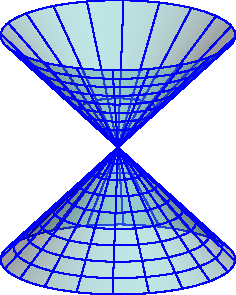
\includegraphics{media/cone.pdf}
	\end{center}

	If we take the standard affine charts now, we obtain the following:
	\begin{itemize}
		\ii At $x=1$, we get a hyperbola $\VV(1+y^2-z^2)$.
		\ii At $y=1$, we get a hyperbola $\VV(1+x^2-z^2)$.
		\ii At $z=1$, we get a circle $\VV(x^2+y^2-1)$.
	\end{itemize}
	That said, over $\CC$ a hyperbola and circle
	are the same thing; I'm cheating a little by drawing $\CC$
	as one-dimensional, just like last chapter.
\end{example}
\begin{ques}
	Draw the intersection of the cone above
	with the $z=1$ plane, and check that you do in fact get a circle.
	(This geometric picture will be crucial later.)
\end{ques}

\section{Homogeneous Ideals}
Now, the next thing we want to do is define $\VV(I)$ for an ideal $I$.
Of course, we again run into an issue with things like $x_0-1$ not
making sense. 

The way out of this is to use only \emph{homogeneous} ideals.
\begin{definition}
	If $I$ is a homogeneous ideal, we define
	\[ \VV(I) = \{ x \mid f(x) = 0 \; \forall f \in I\}. \]
\end{definition}
\begin{exercise}
	Show that the notion ``$f(x) = 0 \; \forall f \in I$''
	is well-defined for a homogeneous ideal $I$.
\end{exercise}
So, we would hope for a nullstellensatz-like theorem
which bijects the homogeneous semiprime ideals to the ideals.
Unfortunately:
\begin{example}
	[Irrelevant Ideal]
	To crush some dreams and hopes, consider the ideal
	\[ I = (x_0, x_1, \dots, x_n). \]
	This is called the \vocab{irrelevant ideal};
	it is homogeneous semiprime
	and has the property that $\VV(I) = \varnothing$.
\end{example}

However, other than the irrelavant ideal.
\begin{theorem}
	[Homogeneous Nullstellensatz]
	Let $I$ and $J$ be homogeneous ideals. 
	\begin{enumerate}[(a)]
		\ii If $\VV(I) = \VV(J) \neq \varnothing$ then $\sqrt I = \sqrt J$.
		\ii If $\VV(I) = \varnothing$, then either $I = (1)$
		or $\sqrt I = (x_0, x_1, \dots, x_n)$.
	\end{enumerate}
	Thus there is a natural bijection between:
	\begin{itemize}
		\ii projective varieties in $\CP^n$, and
		\ii homogeneous semiprime ideas of $\CC[x_1, \dots, x_n]$ 
		except for the irrelevant ideal. 
	\end{itemize}
\end{theorem}
\begin{proof}
	For the first part, let $V = \VV(I)$ and $W = \VV(J)$
	be projective varieties in $\CP^n$.
	We can consider them as \emph{affine varieties} in $\Aff^{n+1}$
	by using the interpretation of $\CP^n$
	as lines through the origin in $\CC^n$.

	Algebraically, this is done by taking the homogeneous ideals
	$I, J \subseteq \CC[x_0, \dots, x_n]$
	and using the same ideals to cut out \emph{affine} varieties
	$V_{\text{aff}} = \VV(I)$ and $W_{\text{aff}} = \VV(J)$ in $\Aff^{n+1}$.
	For example, the cone $x^2+y^2-z^2=0$ is a conic in $\CP^2$,
	but can also be thought of as the two-dimensional cone in $\Aff^3$.

	Then for (a), we have $V_{\text{aff}} = W_{\text{aff}}$,
	so $\sqrt I = \sqrt J$.

	For (b), either $V_{\text{aff}}$ is empty 
	or it is just the origin of $\Aff^{n+1}$,
	so the Nullstellensatz implies either $I = (1)$
	or $\sqrt I = (x_0, \dots, x_n)$ as desired.
\end{proof}


\section{As Ringed Spaces}
\prototype{The regular functions on $\CP^1$ minus a point
are exactly those of the form $P(s/t)$.}
Now, let us make every projective variety $V$ into a baby ringed space.
We already have the set of points, a subset of $\CP^n$.

The topology is defined as follows.
\begin{definition}
	We endow $\CP^n$ with the \vocab{Zariski topology}
	by declaring the sets of the form $\VV(I)$,
	where $I$ is a homogeneous ideal, to be the closed sets.
	
	Every projective variety $V$ then inherits the Zariski
	topology from its parent $\CP^n$.
	The \vocab{distinguished open sets} $D(f)$ are $V \setminus \VV(f)$.
\end{definition}

Thus every projective variety $V$ is now a topological space.
It remains to endow it with a sheaf of regular functions $\OO_V$.
To do this we had to be a little careful.
In the affine case we had a nice little ring of functions,
the coordinate ring $\CC[x_0,\dots,x_n] / I$,
that we could use to provide the numerator and denominators.
So, it seems natural to then define the following:
\begin{definition}
	The \vocab{homogeneous coordinate ring} of a projective variety
	$V = \VV(I) \subseteq \CP^n$, where $I$ is homogeneous semiprime,
	is defined as the ring
	\[ \CC[V] = \CC[x_0, \dots, x_n] / I. \]
\end{definition}
However, when we define rational function we must impose
a new requirement that the numerator and denominator are the same degree.
\begin{definition}
	Let $U \subseteq V$ be an open set of a projective variety $V$.
	A \vocab{rational function} $\phi$ on a projective variety $V$
	is a quotient $f/g$, where $f,g \in \CC[V]$,
	and $f$ and $g$ are homogeneous of the same degree,
	and $\VV(g) \cap U = \varnothing$.
	In this way we obtain a function $\phi : U \to \CC$.
\end{definition}
\begin{example}
	[Examples of Rational Functions]
	Let $V = \CP^1$ have coordinates $(s:t)$.
	\begin{enumerate}[(a)]
		\ii If $U = V$, then constant functions $c/1$
		are the only rational functions on $U$.
		\ii Now let $U_1 = V \setminus \{(1:0)\}$.
		Then, an example of a regular function is
		\[ \frac{s^2+9t^2}{t^2} = \left( \frac st \right)^2 + 9. \]
		If we think of $U_1$ as $\CC$
		(i.e.\ $\CP^1$ minus an infinity point, hence like $\Aff^1$)
		then really this is just the function $x^2+9$.
	\end{enumerate}
\end{example}
Then we can repeat the same definition as before:
\begin{definition}
	Let $U \subseteq V$ be an open set of a projective variety $V$.
	We say a function $\phi : U \to \CC$ is a \vocab{regular function} if
	for every point $p$, we can find an open set $U_p$ containing $p$
	and a rational function $f_p/g_p$ on $U_p$ such that
	\[ \phi(x) = \frac{f_p(x)}{g_p(x)} \qquad \forall x \in U_p. \]
	In particular, we require $U_p \cap \VV(g_p) = \varnothing$.
	We denote the set of all regular functions on $U$ by $\OO_V(U)$.
\end{definition}
Of course, the rational functions from the previous example
are examples of regular functions as well.
This completes the definition of a projective variety $V$
as a baby ringed space.

\section{Examples of Regular Functions}
Naturally, I ought to tell you what the regular functions
on distinguished open sets are; this is an analog to
\Cref{thm:reg_func_distinguish_open} from last time.
\begin{theorem}
	[Regular Functions on Distinguished Open Sets for Projective Varieties]
	Let $V$ be a variety, and let $g \in \CC[V]$ be homogeneous
	of positive degree.
	Then
	\[
		\OO_V(D(g))
		= \left\{ \frac{f}{g^r} \mid
		f \in \CC[V] \text{ homogeneous of degree $r\deg g$}
		\right\}.
	\]
\end{theorem}
What about the case $g = 1$?
A similar result holds, but we need the assumption that $V$ is irreducible.
(This has the same definition as the affine case,
since ``irreducible'' is an adjective of topological spaces.)
\begin{theorem}
	[Only Constant Regular Functions on Projective Space]
	Let $V$ be an \emph{irreducible} projective variety.
	Then the only regular functions on $V$ are constant,
	thus we have \[ \OO_V(V) \cong \CC. \]
\end{theorem}
Proofs of these are omitted for now.
\begin{example}
	[Regular Functions on $\CP^1$]
	Let $V = \CP^1$, with coordinates $(s:t)$.
	\begin{enumerate}[(a)]
		\ii By theorem, if $U_1$ is the standard affine chart
		omitting the point $(1:0)$, we have
		$ \OO_V(U_1) = \left\{ \frac{f}{t^n} \mid \deg f = n \right\} $.
		One can write this as
		\[ \OO_V(U_1) \cong \left\{ P(s/t) \mid P \in \CC[x] \right\}
			\cong \OO_{\Aff^1} (\Aff^1). \]
		This conforms with our knowledge that $U_1$
		``looks very much like $\Aff^1$''.
		\ii As $V$ is irreducible, $\OO_V(V) = \CC$:
		there are no nonconstant functions on $\CP^1$.
	\end{enumerate}
\end{example}

\begin{example}
	[Regular Functions on $\CP^2$]
	Let $\CP^2$ have coordinates $(x:y:z)$ and 
	let $U_0 = \left\{ (x:y:1) \in \CP^2 \right\}$
	be the distinguished open set $D(z)$.
	Then in the same vein,
	\[
		\OO_{\CP^2}(U_0)
		= \left\{ \frac{P(x,y)}{z^n} \mid \deg P = n \right\}
		\cong \left\{ P(x/z, y/z) \mid P \in \CC[x,y] \right\}.
	\]
\end{example}

\section\problemhead
affine and irreducible projective variety not isomorphic unless point


\chapter{Bonus: B\'ezout's Theorem}
In this chapter we discuss B\'ezout's Theorem.
It makes precise the idea that two degree $d$ and $e$
curves in $\CP^2$ should intersect at ``exactly'' $de$ points
In order to make this vision come true:
\begin{itemize}
	\ii We ought to work in $\CP^n$,
	so that for example any two lines intersect.
	\ii We need to account for multiplicities.
	So we will whenever possible work with homogeneous ideals $I$,
	because we want to allow the possibility that $I$ is not semiprime.
\end{itemize}

\section{The Hilbert Function}
Let $I \subseteq \CC[x_0, \dots, x_n]$ be homogeneous.


\chapter{Quasi-Projective Varieties and Regular Maps}
\section{Quasi-Projective Varieties}
Here is yet another type of baby ringed space,
which will turn out to generalize both affine and projective varieties.
\begin{definition}
	A \vocab{quasi-projective variety} is
	an open set $X$ of a projective variety $V$.
	It is a baby ringed space $(X, \OO_X)$ too,
	because for any open set $U \subseteq X$
	we simply define $\OO_X(U) = \OO_V(U)$.
\end{definition}
Obviously, every projective variety is quasi-projective.
But now, we can interpret every affine variety $V$
as a quasi-projective variety by noticing that
\[ V \subseteq \Aff^n \to U_0 \subset \CP^n \]
where $U_0$ is the standard affine chart, isomorphic to $\Aff^n$.

\section{Maps of Baby Ringed Spaces}
In order to make this precise I have to define
what the arrow $\Aff^n \to U_0$ means,
because they are different types of objects;
the former is an affine variety and the latter is a quasi-projective variety.
So, let me actually define a map between \emph{any} baby ringed spaces:
\begin{definition}
	Let $(X, \OO_X)$ and $(Y, \OO_Y)$
	be baby ringed spaces.
	A continuous map of topological spaces $f: X \to Y$
	is a \vocab{regular map} if the following condition holds:
	if $U$ is an open subset of $Y$.
	and $\phi \in \OO_Y(U)$ is regular, then the composition
	\begin{diagram}
		f\pre(U) &\rTo^f & U & \rTo^\phi & \CC
	\end{diagram}
	is a regular function in $\OO_X(f\pre(U))$.

	Two baby ringed spaces are \vocab{isomorphic}
	if there are mutually inverse regular maps between them.
\end{definition}
This is great.
Before this definition, we had three different types of varieties:
\begin{itemize}
	\ii Affine varieties,
	\ii Projective varieties, and
	\ii Quasi-projective varieties.
\end{itemize}
But all three are baby ringed spaces, now they can
talk to each other, and even be isomorphic.
In particular, let's now finally prove:
\begin{proposition}
	[Projective Space is Locally Affine]
	The standard affine chart $U_0$ of $\CP^n$
	is isomorphic to $\Aff^n$.
\end{proposition}
\begin{proof}
	\todo{prove this}
\end{proof}

\end{document}

\section{(Aside) Which rings are coordinate rings?}
As an aside, we might ask: which rings are the coordinate ring of some affine variety?
There are some obvious requirements.
\begin{itemize}
	\ii Such ring must be $\CC$-algebras, of course.
	(A $\CC$-algebra is a ring that contains a copy of $\CC$ in it.)
	\ii Such a ring must be finitely generated, since $\CC[V]$
	is generated by $x_1$, \dots, $x_n$.
\end{itemize}
There is a third more subtle condition.
Define an element $r \in R$ to be \vocab{nilpotent} if $r^N = 0$ for some $r \in R$.
For example, $x$ is nilpotent in $\CC[x]/(x^{2015})$.
Call a ring \vocab{reduced} if it has no nonzero nilpotent elements.

\begin{exercise}
	Let $I$ be an ideal of a ring $R$.
	Show that $I$ is semiprime if and only if $R/I$ is reduced.
\end{exercise}
\begin{remark}
	For a ring $R$, this completes the following table:
	\begin{center}
	\begin{tabular}[h]{l|l}
		Ideal $I$ & Quotient $R/I$ \\ \hline
		Maximal & Field \\
		Prime & Integral Domain \\
		Semiprime & Reduced
	\end{tabular}
	\end{center}
	In particular, $(0)$ is maximal, prime, or semiprime
	if and only if $R/(0) \cong R$ is a field, integral domain, or reduced, respectively.
\end{remark}

Thus, the third requirement is that a coordinate ring must be reduced.
Conveniently, it turns out that these three conditions are sufficient!
\begin{theorem}[Coordinate Rings are Finitely Generated Reduced $\CC$-Algebras]
	Every finitely generated reduced $\CC$-algebra is the coordinate
	ring of some complex affine variety.
\end{theorem}
\begin{proof}
	Let $R$ be this map.
	Because it's finitely generated by some $r_1$, $r_2$, \dots, $r_n$,
	there is some surjective map
	\[ \CC[x_1, \dots, x_n] \surjto R \]
	via $x_i \mapsto r_i$.
	Let $I$ be the kernel of this map.
	Since $R$ is reduced, $I$ is radical.
	Then $R \cong \CC[V]$, where $V = \VV(I)$.
\end{proof}
